\item \points{2a} \textbf{Coding problem: ideal (fully observed) case}

First we will consider the hypothetical (and uninteresting) case, where we have access to the true
$t$-labels for training. In \texttt{src-incomplete/submission.py}, write a logistic
regression classifier that uses $x_1$ and $x_2$ as input features, and train it
using the $t$-labels. More specifically you will implement the |fully_observed_predictions| function.
We will ignore the $y$-labels for this part. Output the
trained model's predictions on the \textbf{test set} to the file specified in the code.

The output plot should look similar to the following (no plot submission is required):
\begin{figure}[H]
	\centering
	\vspace{2mm}
	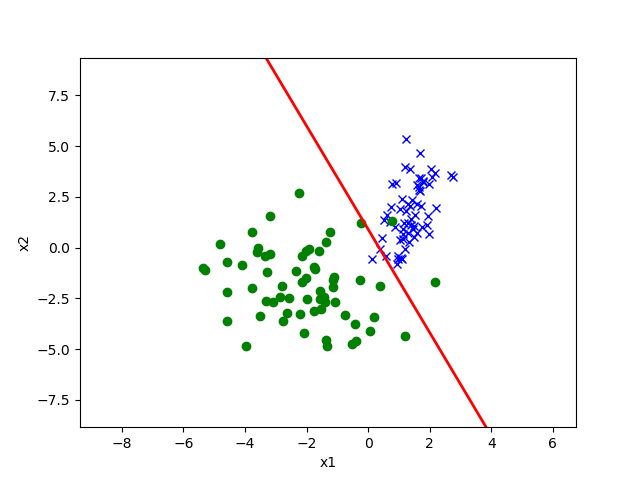
\includegraphics[width=0.5\linewidth]{02-posonly/posonly_true_pred.png}
    \caption{Separating hyperplane for logistic regression on training set using fully observed predictions (Note: This is for reference only.  You are not required to submit a plot.)}
\end{figure}